%Metroplolis Beamer Theme: https://github.com/matze/mtheme
\documentclass[aspectratio=169, 10pt, dvipsnames]{beamer}
\usetheme{metropolis}
\usepackage{appendixnumberbeamer, lmodern, bookmark,fontawesome}
\usepackage{booktabs}
% \usepackage[sorting=none]{biblatex}
\usepackage[scale=2]{ccicons}
\usepackage{pgfplots}
\usepgfplotslibrary{dateplot}
\usepackage{xspace}
\newcommand{\themename}{\textbf{\textsc{metropolis}}\xspace}
\usepackage{bbm}
\usepackage{tikz, graphicx}
\usepackage{caption}
\usepackage{multicol}
% \usepackage[dvipsnames]{xcolor}
\usepackage{animate}
\usepackage{scalerel,xparse}
\usepackage{amsmath}
\usepackage{subfig}
\usepackage{verbatim}
\usepackage{minted}

\newcommand*\colourcheck[1]{%
  \expandafter\newcommand\csname #1check\endcsname{\textcolor{#1}{\ding{52}}}%
}
\colourcheck{blue}

\title{Progress update}
% \subtitle{Lab Update}
\date{\today}
\author{Philip Hartout}

% \titlegraphic{\hfill\includegraphics[height=1.5cm]{logo.pdf}}

\hypersetup{
  colorlinks=true,
  linkcolor=orange,
  filecolor=orange,
  urlcolor=orange,
}

\setminted[python]{fontsize=\tiny}


\def\signed #1{{\leavevmode\unskip\nobreak\hfil\penalty50\hskip1em
  \hbox{}\nobreak\hfill #1%
  \parfillskip=0pt \finalhyphendemerits=0 \endgraf}}

\newsavebox\mybox
\newenvironment{aquote}[1]
  {\savebox\mybox{#1}\begin{quote}\openautoquote\hspace*{-.7ex}}
  {\unskip\closeautoquote\vspace*{1mm}\signed{\usebox\mybox}\end{quote}}

\titlegraphic{%
  
\includegraphics[width=.2\textwidth]{figures/mlcb-transparent.png}\hfill
  
\includegraphics[width=.2\textwidth]{figures/dbsse-transparent.png}\hfill
  
\includegraphics[width=.2\textwidth]{figures/eth-transparent.png}
}

\makeatletter
\setbeamertemplate{title page}{
  \begin{minipage}[b][\paperheight]{\textwidth}
    \vfill%
    \ifx\inserttitle\@empty\else\usebeamertemplate*{title}\fi
    \ifx\insertsubtitle\@empty\else\usebeamertemplate*{subtitle}\fi
    \usebeamertemplate*{title separator}
    \ifx\beamer@shortauthor\@empty\else\usebeamertemplate*{author}\fi
    \ifx\insertdate\@empty\else\usebeamertemplate*{date}\fi
    \ifx\insertinstitute\@empty\else\usebeamertemplate*{institute}\fi
    \vfill
    \ifx\inserttitlegraphic\@empty\else\inserttitlegraphic\fi
    \vspace*{1cm}
  \end{minipage}
}
\makeatother

\usetikzlibrary{shapes.geometric, arrows, chains, positioning, decorations.pathreplacing,decorations.pathmorphing,shapes,%
  matrix,shapes.symbols}

\tikzstyle{orangebox} = [rectangle, very thick, rounded corners, minimum width=2cm, minimum
height=0.5cm, draw=black, fill=YellowOrange!40, minimum height=12mm]
\tikzstyle{bluebox} = [rectangle, very thick, rounded corners, minimum width=2cm, minimum height=0.5cm, draw=black, fill=blue!40]

\tikzstyle{arrow} = [thick,->,>=stealth]


\begin{document}

\maketitle


{
  \setbeamercolor{background canvas}{bg=white}
  \begin{frame}[fragile]{Overview}

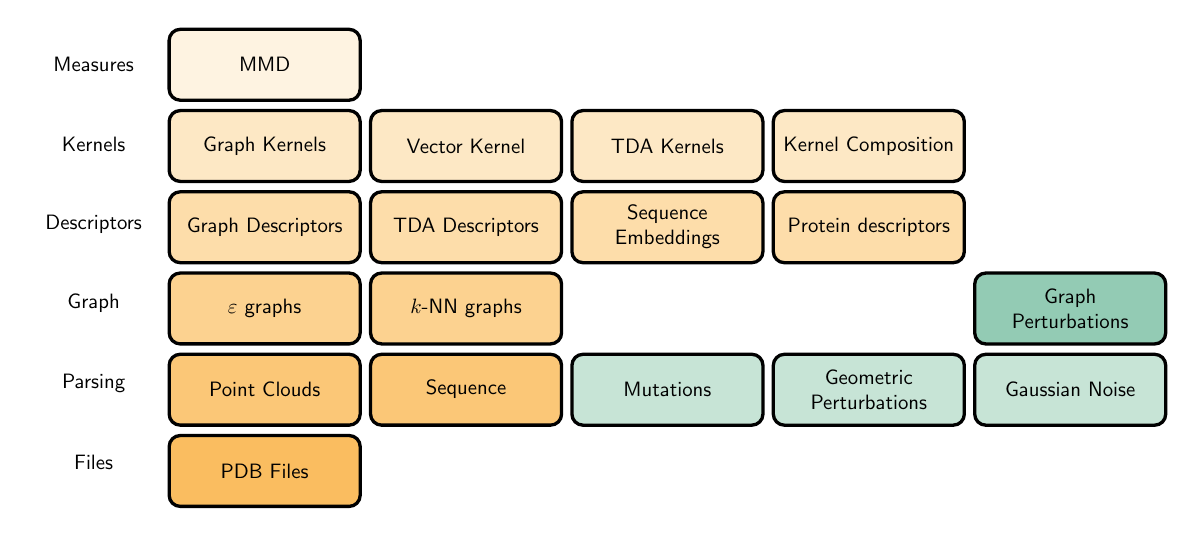
\begin{tikzpicture}[
	scale=0.75,
	start chain=1 going below,
	start chain=2 going right,
	node distance=1mm,
	desc/.style={
		scale=0.75,
		on chain=2,
		rectangle,
		rounded corners,
		draw=black,
		very thick,
		text centered,
		text width=3cm,
		minimum height=12mm,
		fill=blue!30
  },
  % ia/.style={
  %   fill=YellowOrange!10
  % },
  % ib/.style={
  %   fill=YellowOrange!20
  % },
  % ic/.style={
  %   fill=YellowOrange!30
  % },
  % id/.style={
  %   fill=YellowOrange!40
  % },
  % ie/.style={
  %   fill=YellowOrange!50
  % },
  % if/.style={
  %   fill=YellowOrange!60
  % },
	it/.style={
		fill=blue!10
	},
	level/.style={
		scale=0.75,
		on chain=1,
		minimum height=12mm,
		text width=2cm,
		text centered
	},
	every node/.style={font=\sffamily}
]

% Levels
\node [level] (Level 5) {Measures};
\node [level] (Level 4) {Kernels};
\node [level] (Level 3) {Descriptors};
\node [level] (Level 2) {Graph};
% \node [level] (Level 1.5) { };
\node [level] (Level 1) {Parsing};
\node [level] (Level 0) {Files};

% Descriptions
\chainin (Level 5); % Start right of Level 5
% IT levels
\node [desc, fill=YellowOrange!10] (mmd) {MMD};
\node [desc, continue chain=going below, fill=YellowOrange!20] (gkernels) {Graph Kernels};
\begin{scope}[start branch=gkernels]
  \node[desc, on chain=going right, fill=YellowOrange!20](vkernels) {Vector Kernel};
  \node[desc, on chain=going right, fill=YellowOrange!20](tdakernels) {TDA Kernels};
  \node[desc, on chain=going right, fill=YellowOrange!20](tdakernels) {Kernel Composition};
\end{scope}
% ICS levels
\node [desc, fill=YellowOrange!30] (gdescriptors) {Graph Descriptors};
\begin{scope}[start branch=gdescriptors]
  \node[desc, fill=YellowOrange!30, on chain=going right](tdadescriptors) {TDA Descriptors};
  \node[desc, on chain=going right, fill=YellowOrange!30](sequence) {Sequence \\Embeddings};
  \node[desc, on chain=going right, fill=YellowOrange!30](sequence) {Protein descriptors};
\end{scope}
% \node [desc, text width=3.5cm, xshift=-4.5cm] (Graphs2) {$\varepsilon$-graphs 2};
\node [desc, fill=YellowOrange!40] (Graphs) {$\varepsilon$ graphs};
% \node [desc, text width=3.5cm, xshift=4.5cm, on chain=going left] (Graphs2)
% {$\varepsilon$-graphs 2}
\begin{scope}[start branch=Graphs]
  \node[desc, on chain=going right, fill=YellowOrange!40](knn) {$k$-NN graphs};
  \node[desc, on chain=going right, fill=white!100, draw=white](f1) {};
  \node[desc, on chain=going right, fill=white!100, draw=white](f1) {};
  \node[desc, on chain=going right, fill=PineGreen!40](gp) {Graph \\Perturbations};
\end{scope}
\node [desc, xshift=2.25cm, xshift=-2.25cm, fill=YellowOrange!50] (PC) {Point Clouds};
\begin{scope}[start branch=PC]
  \node[desc, on chain=going right, fill=YellowOrange!50](sequence) {Sequence};
  \node[desc, on chain=going right, fill=PineGreen!20](gp) {Mutations};
  \node[desc, on chain=going right, fill=PineGreen!20](gp) {Geometric \\Perturbations};
  \node[desc, on chain=going right, fill=PineGreen!20](gn) {Gaussian Noise};
\end{scope}
\node [desc, fill=YellowOrange!60] (Files) {PDB Files};
% \node [desc, xshift=2.25cm] (IO) {I/O from Sensors};

\end{tikzpicture}
\textcolor{PineGreen!90}{Green: perturbations}\\
\textcolor{YellowOrange!90}{Orange: sequence embeddings}
\end{frame}
}


\begin{frame}[fragile]{Composable transformations \& using
    \texttt{sklearn} API standards sensibly}
  \begin{figure}
    \scalebox{0.75}{
    
\begin{tikzpicture}[align=center, node distance=1.5cm, align=center]
      \node (coords) [orangebox] {Get \\Coordinates};
      \node (cmap) [orangebox, right of=coords, xshift=1.5cm] {Get \\contact map};
      \node (egraph) [orangebox, right of=cmap, xshift=1.5cm] {Get \\$\epsilon$-graph};
      \node (wlk) [orangebox, right of=egraph, xshift=1.5cm] {Compute \\kernel};
      \node (mmd) [orangebox, right of=wlk, xshift=1.5cm] {Compute \\MMD};
      \draw [arrow] (coords) -- (cmap);
      \draw [arrow] (cmap) -- (egraph);
      \draw [arrow] (egraph) -- (wlk);
      \draw [arrow] (wlk) -- (mmd);
    \end{tikzpicture}
  }
  \end{figure}
  \begin{minipage}{.45\textwidth}
    \inputminted{python}{example_pipeline.py}
  \end{minipage}
  \hfill
  \begin{minipage}{.45\textwidth}
    \pause \textbf{What if we now want to add noise?}
  \end{minipage}
\end{frame}

\begin{frame}[fragile]{Composable transformations \& using
    \texttt{sklearn} API standards sensibly}
  \begin{figure}
    \scalebox{0.75}{
    
\begin{tikzpicture}[align=center, node distance=1.5cm, align=center]
      \node (coords) [orangebox] {Get \\Coordinates};
      \node (gauss) [orangebox, right of=coords, xshift=1.5cm] {Add \\gaussian noise};
      \node (cmap) [orangebox, right of=gauss, xshift=1.5cm] {Get \\contact map};
      \node (egraph) [orangebox, right of=cmap, xshift=1.5cm] {Get \\$\epsilon$-graph};
      \node (wlk) [orangebox, right of=egraph, xshift=1.5cm] {Compute \\kernel};
      \node (mmd) [orangebox, right of=wlk, xshift=1.5cm] {Compute \\MMD};
      \draw [arrow] (coords) -- (gauss);
      \draw [arrow] (gauss) -- (cmap);
      \draw [arrow] (cmap) -- (egraph);
      \draw [arrow] (egraph) -- (wlk);
      \draw [arrow] (wlk) -- (mmd);
    \end{tikzpicture}
  }
  \end{figure}
  \begin{minipage}{.45\textwidth}
    \inputminted{python}{example_pipeline.py}
  \end{minipage}
  \hfill
  \begin{minipage}{.45\textwidth}
    \inputminted{python}{example_pipeline_with_noise.py}
  \end{minipage}
\end{frame}

\end{document}
